\documentclass[border=4pt]{standalone}
\usepackage{tikz}
\usetikzlibrary{arrows.meta,positioning,topaths}
\tikzset{
  block/.style={draw,minimum width=22mm,minimum height=9mm,align=center},
  raised route/.style={to path={-- ++(0,10mm) -| (\tikztotarget) \tikztonodes}},
  lowered route/.style={to path={-- ++(0,-10mm) -| (\tikztotarget) \tikztonodes}}
}
\begin{document}
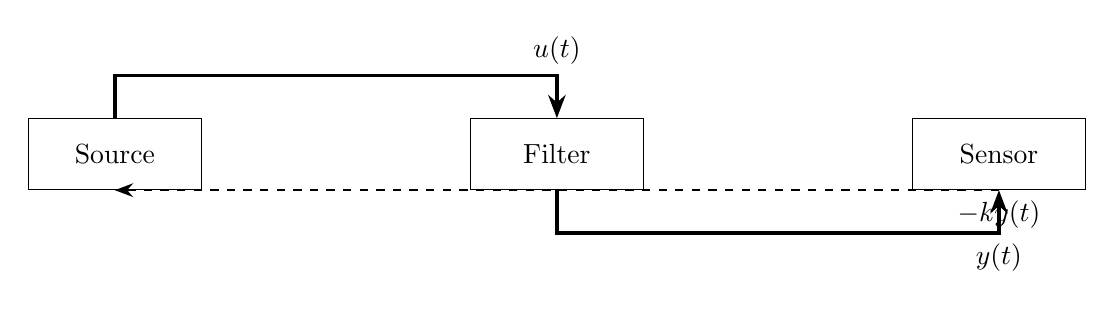
\begin{tikzpicture}[>=Stealth,node distance=34mm]
  \node[block] (source) {Source};
  \node[block,right=of source] (filter) {Filter};
  \node[block,right=of filter] (sensor) {Sensor};
  \draw[->,very thick,raised route] (source) to node[above] {$u(t)$} (filter);
  \draw[->,very thick,lowered route] (filter) to node[below] {$y(t)$} (sensor);
  \draw[->,thick,dashed] (sensor.south) |- node[below] {$-k y(t)$} (source.south);
\end{tikzpicture}
\end{document}
